\section{Architecture générale}
	\subsection{Briques logicielles}
		Notre projet peut être séparé en plusieurs briques logicielles ; celles-ci correspondent à une première ébauche de l'architecture globale du programme.
		\subsubsection{Moteur de rendu : Unity}
			La première brique est Unity; nous l'utiliserons ici pour sa composante moteur de jeu et environnement de développement, et non pour ses fonctionnalités de création d'objets 3d, de modélisation, de génération de codes et de gestion d'entrées-sorties.
		\subsubsection{Gestion des périphériques : MiddleVR}
			La gestion des périphériques est réalisée par MiddleVR ; l'avantage de celui-ci par rapport à la fonctionnalité native d'Unity est la grande flexibilité de la gestion des périphériques ; qui permet de déployer l'application sur des plateformes très diverses et de centraliser les périphériques.
		\subsubsection{Interactions avec les objets}
			Nous allons devoir développer un système d'interactions entres les objets, pour qu'une action sur un objet ait un effet sur un autre objet.
		\subsubsection{Gestion des scénarios}
			Les scénarios demandés dans le cahier des charges devront être implémentés ; il pourrait être appréciable que de nouveaux scénarios puissent facilement être ajoutés.
			De ce fait, nous avons besoin d'un système de gestion des scénarios qui devra par exemple donner l'ordre de différentes actions à réaliser par l'utilisateur, et d'éventuelles aides supplémentaires s'il devait réaliser une action autre que celle demandée.
		\subsubsection{Gestions des objets manipulables}
			Nous devrons aussi implémenter de quoi gérer les objets, pour pouvoir les retrouver et les gérer dans l'espace.
		\subsubsection{Menu}
			Un menu devra être disponible au lancement de l'application, ainsi qu'au cours de l'utilisation.

%-------------------------------------------------------------------------------------------------------
%
%							Partie 4.2
%
%-------------------------------------------------------------------------------------------------------
\subsection{Liens entre les modules}
Dans cette partie, nous détaillons comment différentes entités du logiciel sont reliées, pour définir comment elles vont fonctionner entre elles.

\subsubsection{Middle VR et Unity}
Comme nous l'avons vu précédemment, MiddleVR permet de gérer différents types de périphériques d'interfaces utilisateur, allant du traditionnel couple souris/clavier aux manettes de jeu les plus perfectionnés.
Unity, qui est le moteur 3D, reçoit les commandes des périphériques sus-nommés, et permet ainsi d'agir avec la scène.
Le problème est que l'on ne peut pas redéfinir toutes les interactions pour chaque type de contrôleur sous Unity : il faudrait tout refaire pour un nouveau périphérique.
Nous allons utiliser MiddleVR pour abstraire notre modélisation Unity, et s'occuper de récupérer les signaux des contrôleurs de jeu. Unity récupère les données nécessaires via MiddleVR.
Ainsi pour chaque nouveau périphérique, il suffit juste de modifier le comportement de MiddleVR pour l'utiliser sous Unity sans rien changer.
Cela en fait une implémentation très générique (presque) indépendante du matériel utilisé.
MiddleVR gère l'interface avec VRPN, un protocole standard client/serveur de haut niveau qui permet de gérer de très nombreux périphériques de réalité virtuelle.

\subsubsection{Gestionnaire d'objets et objets}

Dans la modélisation de l'appartement, il y a un certains nombre d'objets avec lesquels l'utilisateur pourra interagir.
Or, ces interactions se feront via un \enquote{gestionnaire d'objet}.
En effet, l'action sur un objet pouvant se répercuter sur d'autres objets, ou varier suivant le contexte logiciel (mode, scénario ...), il faut un gestionnaire d'objet pour exploiter toutes les possibilités qui s'offrent à nous.
Il sera codé \enquote{à côté d'Unity}, c'est à dire qu'il le complétera et sera intégré après modélisation (pas besoin de modifier la modélisation pour changer les comportements).

La communication entre ces deux entités doit pouvoir se faire dans les deux sens.
En effet, imaginons le cas d'un interrupteur : si l'utilisateur appuie sur un bouton, on aimerait que l'action qui y est associée soit effectuée (allumer lampe, baisser volets etc ...).
Pour faire cela, on va transmettre à une autre entité l'action qui s'est exécutée sur l'objet : le gestionnaire d'objet.
C'est alors le gestionnaire qui va analyser l'action et son contexte et exécuter le code approprié. C'est le premier sens de communication, c'est à dire de l'objet vers le gestionnaire d'objets.
Une fois la situation analysée et la décision prise, le gestionnaire peut avoir à répercuter une action sur un objet afin d'en modifier l'état (allumer/éteindre un objet lampe).
C'est le deuxième sens de communication, c'est à dire du gestionnaire vers l'objet.

\subsubsection{Gestionnaire de scénario et gestionnaire d'objet}

Sur le même principe que précédemment, les liens entre objets peuvent varier suivant les scénarios et modes d'apprentissage.
Par exemple on peut désactiver toutes les fonctions des stores électriques pour le mode assisté, mais les activer pour le mode autonome.
On peut aussi décider de désactiver tel ou tel objet pour un scénario en particulier, c'est pourquoi nous allons passer par un \enquote{gestionnaire de scénario}.
La communication entre les deux est nécessairement bilatérale : en effet on peut imaginer que le gestionnaire de scénario instancie un gestionnaire d'objet en particulier et attend des ordre pour la validation des objectifs par exemple.

\subsubsection{Récapitulatif}
\begin{figure}
	\centering
		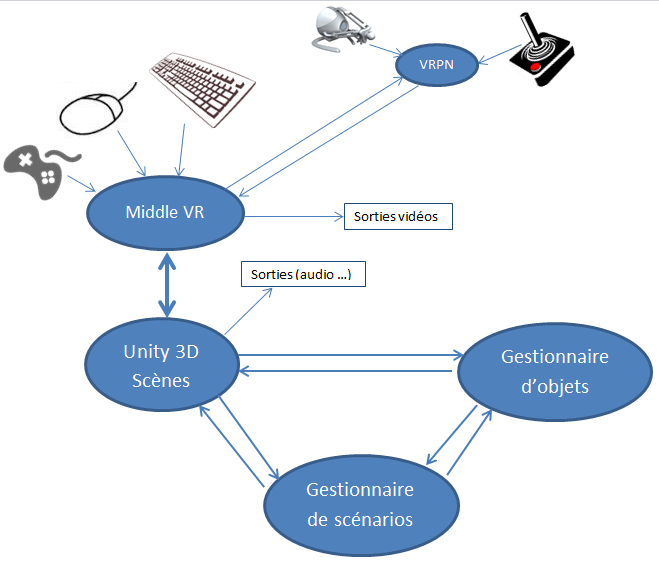
\includegraphics[width=\textwidth]{2-Specifications/img/recap.png}
		\caption{Récapitulatif des interactions entre briques logicielles}
	\label{fig:unityvr}
\end{figure}


%MiddleVR <=> Unity
%Gestionnaire d’objets <=> Objets
%Gestionnaire scénarios <=> Gestionnaire d’objets
